\documentclass[12pt]{article}
\usepackage{arxiv}
\usepackage[english, russian]{babel}
\usepackage[T1]{fontenc}
\usepackage{url}
\usepackage{booktabs}
\usepackage{amsfonts}
\usepackage{nicefrac}
\usepackage{microtype}
\usepackage{lipsum}
\usepackage{graphicx}
\usepackage{natbib}
\usepackage{doi}
\usepackage[unicode, pdftex]{hyperref}
\usepackage[utf8]{inputenc}
\usepackage{amsmath}
\usepackage{mathtools}
\usepackage{algpseudocode}
\usepackage[margin=3cm]{geometry}
\usepackage{algorithm2e}
\usepackage{ dsfont }

\usepackage{setspace}
\singlespacing % полуторный интервал для всего текста


\title{Дистилляция моделей и данных}

\author{ Баринов Никита\\
	МФТИ\\
	\And
	Филатов Андрей \\
	МФТИ       
}
\date{}

\renewcommand{\undertitle}{}
\renewcommand{\headeright}{}
\renewcommand{\shorttitle}{Дистилляция моделей и данных}

\hypersetup{
pdftitle={Дистилляция моделей и данных},
pdfauthor={Баринов Никита},
pdfkeywords={Deep Learning \and Distilling the Knowledge \and Dataset Distillation},
}

\begin{document}
\maketitle

\begin{abstract}

%отдельно про дистилляцию моделей - сократить размер модели
%данных - обучить две модели можем
% не сущ-т решения одновременной 
% провели рез-ты и получили качество не сильно хуже

    Во многих задачах ML точность предсказания модели зависит от её размера. При этом зачастую данная зависимость выглядит достаточно тривиально: последовательное увеличение размеров модели позволяет последовательно улучшать точность её предсказаний. Но такой безграничных рост приводит к ряду проблем: существенное увеличение времени обучения, высокие требования к размерам и качеству обучающей выборки, а также вычислительные сложности. Аналогичная проблема и с данными: чем их больше, тем дольше модель на них обучается.
    В связи с этим возникает желание одновременно <<сжать>> и данные, и модели так, чтобы на новых данных модель меньшего размера не сильно теряла в качестве. Этот процесс называется дистилляцией моделей и данных, и в статье мы предлагаем одно из решений. Вычислительные эксперименты проводятся на выборке изображений CIFAR10. 


\end{abstract}

\keywords{Deep Learning \and Distilling the Knowledge \and Dataset Distillation \and Model Compression}


\section{Introduction}

Глубокое обучение добилось огромного успеха за последние несколько лет в различных областях, таких как компьютерное зрение, обработка естественного языка и распознавание речи. Но всё это требует большиие вычислительные и временные ресурсы.

Со временем начали появляться методы <<сжатия>> моделей без сильной потери качества. Появился термин дистилляция знаний(knowledge distillation) – это способ обучения в первую очередь нейросетевых моделей машинного обучения, направленный на передачу знаний от модели-учителя к модели-ученику. Данная проблема происходит из следующих соображений. Много раз было замечено, что в широком диапазоне практически значимых задач машинного обучения точность предсказания модели существенно зависит от её размера. При этом зачастую данная зависимость выглядит очень просто: последовательное увеличение размеров модели позволяет последовательно улучшать точность её предсказаний. Однако такой безграничный рост приводит к ряду проблем, связанных с практическим применением итоговых моделей. Первой статьёй, в которой можно встретить дистилляцию знаний в современном виде является \cite{hinton2015distilling}.

Поскольку проблема есть и с большим объёмом денных, появился термин дистилляция данных(dataset distillation) - это существенное уменьшение выборки, путём создания искусственных объектов (синтетических данных), которые агрегируют полезную информацию, хранящуюся в данных, и позволяют настраивать алгоритмы машинного обучения не менее эффективно, чем на всех данных. Но почему дистилляция наборов данных полезна, ведь кажется, что мы теряем большую часть информации? Итак, если мы имеем лишь несколько достаточно хорошо дистиллированных изображений, мы можем гораздо эффективнее обучить нейронную сеть на целом наборе данных,
по сравнению с традиционным обучением, при котором часто используются десятки тысяч шагов градиентного спуска. Каждый элемент синтетических данных содержит в себе больше информации, чем отдельный элемент исходной выборки. Например, в нашей работе на выборке CIFAR10 каждому классу соответствует ровно один элемент дистиллированной выборки.

В данной работе предлагается новый подход: одновременная дистилляция модели и данных методами \cite{hinton2015distilling} и \cite{cazenavette2022dataset}. Предлагается сначала сжать информацию, затем обучить на новых синтетических данных большую модель, а затем дистиллировать её. Поставлена оптимизационная задача, реализован предложенный метод и проведено сравнение с уже существующими. Все вычислительные эксперименты проводятся на выборке CIFAR10. 

\section{Related works}

 Сегодня существует несколько решений проблемы дистилляции моделей или данных в отдельности. 

\subsection{Дистилляция моделей}
%применили дистилляцию чтобы сжать модель ансамбль в одну модель
В статье \cite{romero2014fitnets} говорится, что активации, нейроны или особенности слоев могут также использоваться для обучения меньшей модели. Ещё один способ дистилляции, описанный в статье \cite{ba2014deep}, он основан на том, что меньшая модель(ученик) обучается аналогично большей(учитель), тем самым получается конкурентоспособная производительность. В \cite{hinton2015distilling} применили дистилляцию, чтобы сжать ансамбль в одну модель. Одной из последних работ является \cite{chung2020feature}. В ней описывается дистилляция в онлайн-режиме: модель и ученик совместно оптимизируются на каждой итерации. Также существует кросс-модельная дистилляция(передача знаний между промежуточными моделями), одним из сценариев котороя является \cite{chen2021learning}: имеется граф взаимоотношений между моделями, а передача знаний осуществляется при помощи предложенной функции потерь, сохраняющей локальность.

%найти поновее статьи, страница 11, multi-teacher дистилл.



\subsection{Дистилляция данных}
%порядок статей временной
Например, сначала данные инициализируются случайным шумом, а затем при помощи градиентного спуска происходит обновление синтетических данных. Эта процедура подробнее описана в \cite{wang2018dataset}. Описанный метод имеет явный недостаток: он ограничен числом эпох обучения. Использование теоремы о неявной функции в \cite{lorraine2020optimizing} помогает избавиться от такого недостатка. В \cite{zhao2020dataset} в качестве функции ошибки используется расстояние между градиентами этой ошибки по параметрам ученика, которые получаются при обучении на обычных и дистиллированных данных. Альтернативным вариантом может быть введение генеративной модели(может создавать новые данные, которые похожи на те, что были использованы для ее обучения), способной из шума и меток класса создавать необходимые для обучения синтетические изображения, этот подход подробно описан в \cite{such2020generative}.
Статья \cite{cazenavette2022dataset} предлагает метод дистилляции путем создания выборки, на которой динамика обучения такая же, как и на исходной.
%почему теорема о неявной функции полезна
%ванг ограничен числом эпох, а эти ограничения обошлись применением теоремы о неявной функции
%жао в кач-ве ф.ош.  исп расст....


%абстрактная вещь в начале дип лернинг чето там
%подвод к дистилляции данных, в чем прикол, позволит обечать модели намного быстрее и тд
%во многих задачах модели сильно избыточные, и для того чтобы сохранить кач-во и обобщ спос большой модели применяется подходит дистилляции моделей
% в чем вклад: предложили то то то
%в методее рассм применение, как можно примениь на релаьных задачах



\section{Постановка проблемы}

%два аргмина: модель: лосс

В этом разделе описывается предлагаемое решение: дистилляция данных, затем обучения модели на синтетических данных, и дистилляция самое модели. Для этого предлагается поставить две оптимизационные задачи.

Пусть $\mathcal{D}_{real} = \{(\mathbf{x_i}, y_i)\}_{i = 1}^N$ --- исходная выборка. Наша задача --- создать меньшую выборку $\mathcal{D}_{syn} = \{(\mathbf{x_i}, y_i\}_{i = 1}^M$, где $M \ll N$ и такой, что качество модели, обученной на нём похоже на качество при обучении на исходных данных. Наш метод дистилляции предполагает создание экспертных траекторий обучения $\tau^*$, под которыми понимается последовательность параметров $\{ \theta_t^*\}_{t = 0}^T$, полученных во время обучения нейронной сети на $\mathcal{D}_{real}$. Чтобы получить экспертные траектории, предлагается обучить большое количество нейронных сетей на $\mathcal{D}_{real}$ и сохраним их параметры на каждой эпохе. Также определим $\hat\theta_t$ - параметры модели-студента, обученной на $\mathcal{D}_{syn}$ на шаге обучения $t$. На каждом шаге обучения мы будем выбирать случайно $\theta_t^*$, инициализировать этим значением парметры модели-студента $\theta^*_t := \theta_t^*$. Установим верхнюю границу $T^{max}$ на число $t$, чтобы игнорировать ту часть обучения, где параметры меняются незначитально. 

Пусть $l(\mathcal{A}(\mathcal{D}_{syn}), \theta_t)$ - дифференцируемая функция потерь, $\mathcal{A}$ - дифференцируемая техника аугментации данных(это метод, используемый в машинном обучении, для увеличения размера обучающего набора данных путем создания новых примеров на основе существующих данных.) \cite{romero2014fitnets}. После инициализации параметров модели-студента мы совершим $N$ шагов градиентного спуска по параметрам $\hat\theta_t$:
\[
\hat\theta_{t+n+1} = \hat\theta_{t+n} - \alpha\nabla l(\mathcal{A}(\mathcal{D}_{syn}), \hat\theta_{t+n}),
\eqno(1)
\]

где $\alpha$ - шаг обучения модели-студента, используемый для обновления её параметров. 
После обучения градиентного спуска для конкретной траектории $\tau^* \in \{\tau_i^*\}$ считаем 
\[
\mathcal{L} = \frac{\parallel\hat\theta_{t+N}-\theta_{t+M}^*\parallel_2^2}{\parallel\theta_t^* - \theta_{t+M}^* \parallel_2^2},
\eqno(2)
\]

где $\mathcal{L}$ - функция потерь между конечными параметрами студента и учителя, нормированная на пройденное учителем расстояние, что помогает получать информацию о более поздних стадиях его обучения, где параметры меняются не сильно. В конце мы обновляем $\mathcal{D}_{syn}$ в соответствии с обучаемым параметром $\alpha$ и посчитанной функцией $\mathcal{L}$. Итоговый алгоритм выглядит так:

\RestyleAlgo{ruled}
%% This is needed if you want to add comments in
%% your algorithm with \Comment
\SetKwComment{Comment}{/* }{ */}
\begin{algorithm}[hbt!]
\caption{Data Distillation}\label{alg:two}
\KwData{\{\tau_i^*\} - \text{множество параметров учителей, обученных на }\mathcal{D}_{real}}
\KwData{$M$ - \text{число обновлений между стартовыми и целевыми параметрами учителя}}
\KwData{$N$ - \text{число обновлений студента за один шаг дистилляции}}
\KwData{$\mathcal{A} - \text{дифференцируемая функция аугментации}$}
\KwData{$T^{max} < T - \text{максимальная стартовая эпоха}$}
\KwResult{\text{Дистиллированный набор } $\mathcal{D}_{syn}$ и $\alpha$}
$\mathcal{D}_{syn} \gets \mathcal{D}_{real}$\;
$\alpha \gets \alpha_0$\;
\For{$step : 1 \ .. \ N$}{
  $\tau^* \sim \{\tau_i^*\}, \tau^* = \{\theta_t^*\}_0^T$ - \text{выбираем траекторию обучения}\;
  $t \leq T^*$ - \text{случайно выбираем начальную эпоху}\;
  $\theta^*_t := \theta_t^*$ - \text{инициализируем веса студента параметрами учителя}\;
  \For{$n : 0 \ .. \ N-1$}{
    $b_{t+n} \sim \mathcal{D}_{syn}$ - \text{выбрать мини-батч из }$\mathcal{D}_{syn}$\;
    $\hat\theta_{t+n+1} \gets \hat\theta_{t+n} - \alpha\nabla l(\mathcal{A}(\mathcal{D}_{syn}), \hat\theta_{t+n})$\;
  }
  $\mathcal{L} \gets \parallel\hat\theta_{t+N}-\theta_{t+M}^*\parallel_2^2 / \parallel\theta_t^* - \theta_{t+M}^* \parallel_2^2$\;
  \text{Изменить } $\mathcal{D}_{syn}$ \text{ и } $\alpha$ \text{ в зависимости от } $\mathcal{L}$\;
  }
\end{algorithm}


Итого первая оптимизационная задача, которая решает дистилляцию данных, выглядит так:
\[
\mathbf{\hat X}, \alpha = \underset{\mathbf{x}, \alpha}{\arg\min}~ l(\mathbf{x}, \alpha, \theta), \ \mathcal{D}_{syn} = \underset{\mathbf{\hat x} \in \mathbf{\hat X} }{\bigcup}~\mathbf{\hat x}.
\eqno(3)
\]

Далее стоит задача обучения нейросети на дистиллированных данных $\mathcal{D}_{syn}$ и дистилляция модели. 

$\mathbf{Def \ 1:}$ Дистилляция модели - снижение сложности модели путем выбора модели в множестве более простых моделей на основе анализа пространства параметров и предсказаний целевой перменной более сложной фиксированной модели.

$\mathbf{Def \ 2:}$ Учитель - фиксированная модель, ответы которй используются при выборе модели-ученика.

$\mathbf{Def \ 3:}$ Ученик - модель, которая выбираемся согласно заданному критерию качества учителя.

Итак, решается задача класификации:
\[
\mathcal{D} = \{ (\mathbf{\hat x_i}, y_i) \}_{i=1}^R,
\]
где $y_i \in \mathds{Y} = {1,2,...,R}$, $R$ - число классов, $\mathbf{\hat x_i} \in \mathds{R}^n$.

В дистилляции Хинтона \cite{hinton2015distilling} рассматривается параметрическое семейство функций:
\[
\mathcal{G} = \{\mathbf{g} \ | \ \mathbf{g} = softmax(\mathbf{z}(\mathbf{x})/T), \ \mathbf{z}: \mathds{R}^n \rightarrow{} \mathds{R}^R\},
\eqno(4)
\]
где $\mathbf{z}$ - дифференцируемая параметрическая функция заданной структуры, $T$ - параметр температуры. В качестве модели-учителя рассматривается функция $\mathbf{f}$ из множества:
\[
\mathcal{F} = \{\mathbf{f} \ | \ \mathbf{f} = softmax(\mathbf{v}(\mathbf{x})/T, \ \mathbf{v}: \mathds{R}^n \rightarrow{} \mathds{R}^R  \},
\eqno(5)
\]
где $\mathbf{z}$ - дифференцируемая параметрическая функция заданной структуры, $T$ - параметр температуры. 

При этом температура $T$ имеет свойства:

\begin{enumerate} 
\item при Т $\rightarrow 0$ получаем вектор, в котором один из классов имеет единичную вероятность;
\item при Т $\rightarrow \infty$ получаем вектор, в котором все классы равновероятны.
\end{enumerate} 

Функция потерь $\mathcal{L}$ учитывает перенос инфорации от модели-учителя $\mathbf{f}$ к ученику $\mathbf{g}$ и имеет вид:

\[
\mathcal{L}(\mathbf{g}) = - \sum\limits_{i=1}^m \sum\limits_{r=1}^R y_i^r \log\mathbf{g}(\mathbf{x_i}) \bigg|_{T=1} - \sum\limits_{i=1}^m \sum\limits_{r=1}^R \mathbf{f}(\mathbf{x_i}) \bigg|_{T=T_0} \log\mathbf{g}(\mathbf{x_i}) \bigg|_{T=T_0},
\eqno(6)
\]

где первое слаагемое отвечает за исходную функцию потерь, а второе - за дистилляцию. Итого получаем оптимизационную задачу:
\[
\mathbf{\hat g} = \underset{\mathbf{g} \in \mathcal{G}}{\arg\min}~\mathcal{L}(\mathbf{g}).
\eqno(7)
\]

% дистилляция моделей, acc на тесте mnist, описать параметры все эпохи, опт ...
% resnet50-teacher, resnet18-student. pretrained=False. torchvision.models.resnet18
% поменять число каналов на 1
% итог - две цифры два аккураси
% логгер: импорт самари райтер и во время обучения записывать в него
% таблица(-цы)
%

\section{Эксперимент}

\subsection{Базовый эксперимент}

Проведем базовый эксперимент на выборке CIFAR10, с которым будем сравнивать результаты в дальнейшем: дистилялция моделей. Для этого в качестве модели-учител используем $ResNet50$, в качестве модели-ученика $ResNet18$. 

\begin{table}[htbp]
  \centering
  \begin{tabular}{|c|c|c|}
    \hline
    Модель & Число эпох & Accuracy \\ \hline
    ResNet18 & 8 & 74.01\% \\ \hline
    ResNet50 & 8 & 74.83\% \\ \hline
  \end{tabular}
  \caption{Точность моделей в отдельности}
  \label{tab:my-table}
\end{table}

Зависимоть функции потерь и точности от эпохи обучения для каждой модели в отдельности можно видеть на графиках:

\begin{figure}[h]
\centering
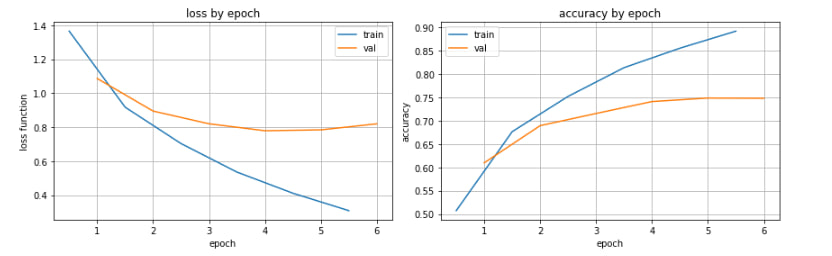
\includegraphics[width=1\textwidth]{resnet50lrcurve.jpg}
\caption{Процесс обучения ResNet50}
\label{fig:имя_файла}
\end{figure}

\begin{figure}[h]
\centering
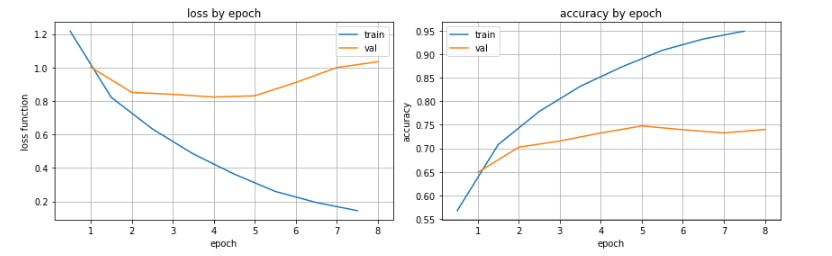
\includegraphics[width=1\textwidth]{resnet18lrcurve.jpg}
\caption{Процесс обучения ResNet18}
\label{fig:имя_файла}
\end{figure}

\newpage
Теперь используем дистилляцию моделей, результаты представлены в таблице:

\begin{table}[htbp]
  \centering
  \begin{tabular}{|c|c|c|c|}
    \hline
    Distillation weight & Функция потерь & Число эпох & Accuracy \\ \hline
    0.25 & $0.75\cdot CrossEntropy+0.25\cdot KLloss$ & 3 & 70.76\% \\ \hline
    0.5 & $0.5\cdot CrossEntropy+0.5\cdot KLloss$ & 3 & 73.02\% \\ \hline
    0.75 & $0.25\cdot CrossEntropy+0.75\cdot KLloss$ & 3 & 75.32\% \\ \hline
  \end{tabular}
  \caption{Дистилляция моделей}
  \label{tab:my-table}
\end{table}

\textbf{Вывод:} дистилляция моделей улучшила качество модели-ученика.



\subsection{Основной эксперимент}




\newpage
\bibliographystyle{unsrt}
\bibliography{ref}

\end{document}